\chapter{Estado del arte} \label{ch:estado}

A lo largo de este capítulo y a la vez del documento, se expondrá de forma sencilla y concisa, el concepto de monitorización, por el cual podemos encontrar los diferentes tipos de herramientas que nos ayudarán a realizar una monitorización exhaustiva del elemento que queremos examinar con exactitud, esto lo iremos elaborando y trabajando en este Trabajo Fin de Grado (TFG).

Veremos las herramientas actuales en el mercado y tras seleccionar la más apropiada para nuestro caso, entraremos en detalle del funcionamiento, el despliegue de la herramientas y las pruebas a realizar, todo esto irá explicado en los próximos capítulos.

\section{Monitorización}

A la hora de hablar sobre el concepto de \textbf{monitorización} de sistemas, tenemos que introducirnos en un concepto que nace con el objetivo de realizar un control exhaustivo sobre la red y los dispositivos que la integran de tal forma que se puedan gestionar las incidencias que vayan ocurriendo con el tiempo de una forma más rápida y eficaz.

Podemos encontrarnos ante el concepto de \textbf{monitorización proactiva}, que se trata de aquella en la que se toman las medidas preventivas y consecuentes con la información que se obtienen de todos los dispositivos que se encuentran conectados a una red, para evitar posibles eventos que hacen que se interrumpan el correcto funcionamiento de alguno de ellos.
\newpage
Para poder abordar este concepto se utilizan protocolos que permitan la comunicación de la red con la herramienta. 

Como estaremos analizando sistemas o cualquier dispositivo donde toda la información relevante será enviada a través de la red, será importante aplicar el uso del protocolo \textbf{SNMP} \cite{snmp}.

\textbf{SNMP}, sus siglas vienen de la palabra en inglés Simple Network Management Protocol, este protocolo pertenece a la capa de aplicación del modelo ISO, y como hemos mencionado permite el intercambio de información amplia sobre los diferentes dispositivos de red.

Este protocolo tiene dos formas de funcionar, la primera forma recibe el nombre de \textbf{polling} y la segunda forma recibe el nombre de \textbf{traps}.

El \textbf{polling} consiste en lanzar consultas de forma remota ademas de forma activa o demanda, realizando una operación síncrona de consulta. Los \textbf{traps} son mensajes que envían los dispositivos SNMP a una dirección configurada basándose en cambios o eventos, de forma asíncrona.\cite{polling}
\subsection{Ventajas y desventajas de SNMP}
La \textbf{principal ventaja} de \textbf{SNMP} es que es un estándar abierto. Los protocolos abiertos están diseñados para combatir el esfuerzo y los costos desperdiciados cuando un fabricante desarrolla su propio protocolo "patentado" que solo soportará.

Las \textbf{desventajas de SNMP} son tales que al poder obtener cualquier dato como una IP (ya sea una IP fuente o una IP destino), una MAC, un puerto o un protocolo, hacen que su utilidad su utilidad se encuentre limitada a lo anterior descrito, ya que no facilita un procesamiento del tráfico, ni una obtención de datos más complejos sobre cualquier red. Por lo que la visibilidad se encontraría considerablemente reducida a las posibilidades de las consultas.

Se encuentra vinculada con cualquier estándar de comunicaciones poco utilizado. Aún así, el lanzamiento de SNMPv3 agregó nuevas opciones de cifrado y privacidad que nunca antes habían existido dentro de SNMP. 

\textbf{SNMP} es un protocolo bastante detallado. Los mensajes detallados se envían entre dispositivos, no solo pequeños códigos preestablecidos. Este inconveniente se ha vuelto bastante pequeño en la mayoría de las aplicaciones, ya que el ancho de banda se ha disparado en los últimos años.

Actualmente, existen múltiples herramientas capaces de realizar la tarea de monitorización a través de aplicaciones o software que se encargan de la monitorización de cualquier red, dispositivo o sistema.

En el punto siguiente llevaremos a cabo una comparativa entre las posibles herramientas que podemos encontrar, basándonos en la documentación ofrecida por sus páginas oficiales de producto.

Existen una gran cantidad de herramientas, en este documento solo vamos a explicar las que se encuentran al alcance de cualquiera, por lo que nos será de preferencia comparar herramientas \textbf{OpenSource}.

Una herramienta \textbf{OpenSource} destaca por el hecho de que cuenta con la posibilidad de compartirse, modificarse y estudiarse su código abierto con la licencia que permite al usuario acceder a él con total libertad.

Realizaremos una enumeración de las más importantes, añadiendo además sus ventajas y desventajas de cada una y realizando la correspondiente \textbf{comparativa}.
\section{Comparación herramientas de monitorización OpenSource}
Las \textbf{herramientas de monitorización} se caracterizan unas de otras, por la manera en que realizan el intercambio de información entre los dispositivos. Por ello, en este apartado se destacará de las principales herramientas, los aspectos que las hacen destacar frente a otras y las carencias que estas presentan.

Estas aplicaciones deberían poder darnos la facilidad de encontrar la información acerca de cualquier dispositivo incluido dentro de la red o cualquiera de los componentes en tiempo real.

Entre estos componentes podemos encontrar servidores físicos o virtuales, servicios de correo, routers, switches, medición de protocolos, etc.

Hay que tener en cuenta que las redes y nuevas tecnologías van avanzando de forma exponencial, por lo que estas herramientas también deben ser capaces de adaptarse a este proceso de evolución. 
\newpage
La mayoría permitirán mostrarlo de forma gráfica con su propio entorno o con la ayuda de herramientas que cuentan con \textbf{interfaz GUI}, dicho término corresponde a la interfaz gráfica de usuario que es un tipo de interfaz de usuario que utiliza imágenes, iconos y menús para mostrar las acciones disponibles entre las que el usuario puede escoger en un dispositivo. 

Su función es proporcionar un entorno visual amigable y sencillo de usar que facilite la comunicación del usuario con el equipo.

Una de sus utilidades es que nos ayudará a mostrar todos los mecanismos necesarios y visuales para nosotros y así mostrarnos con mayor facilidad cualquier problema.

\subsection{Zabbix}
\begin{figure}[H]
	\centering
	
\includegraphics[scale=0.8]{imagenes/logos_monitorizacion/zabbix.png}
	\caption{Zabbix} \label{zabbix}
\end{figure}
\textbf{Zabbix} \cite{zabbix} surge en 2001. Se trata de desarrollo completo,  y su principal característica es que tiene una visión más holística de la monitorización, cubriendo rendimiento, no solo estados, ya que esta es una de las carencias más significativas de algunas herramientas de monitorización. Además de disponer de un sistema de gestión WEB que permite gestionarlo de forma centralizada, sin problemas en los ficheros de configuración.

Puede controlar aspectos como carga del dispositivo, actividad en la red, parámetros del sistema operativo, etc. Además ofrece la posibilidad de generar
informes y gráficas en su interfaz web desarrollada en \textbf{PHP y JavaScript}.
\newpage
Todo su contenido, capaz de recopilar datos de
servidores y aplicaciones, por medio de agentes instalados
en las máquinas cliente, se encuentran desarrollados en C. Soporta casi todos los  \textbf{sistemas de gestión de bases de datos (SGBD)} desde MySQL, PostgreSQL, SQLite, Oracle o IBM DB2.

\textbf{Zabbix} tiene una interfaz web de gestión y que ésta se halla centralizada a través de la base de datos.

Posee un sistema de alertas para envío de notificaciones a través de email o SMS, pero además añade el uso de \textbf{Extensible Messaging Presence Protocol(XMPP)}\cite{xmpp}(antes llamado Jabber), encargado de soportar mensajería instantánea, basado en \textbf{XML}.

Posee la ventaja de \textbf{detectar nuevos elementos añadidos a la red y puede establecer una jerarquía entre ellos}.
Sin embargo, la capacidad de esta herramienta viene limitada a un número total de 1.000 nodos y hace que no esté a la misma altura que otras herramientas de características similares.

Otra desventaja es que no puede crear informes en tiempo real, además de no garantizar la seguridad SSL \cite{ssl}.

\subsection{Cacti}
\begin{figure}[H]
	\centering
	
\includegraphics[scale=0.8]{imagenes/logos_monitorizacion/cacti.png}
	\caption{Cacti} \label{cacti}
\end{figure}
\textbf{Cacti} \cite{cacti} \textbf{recopila información de los sistemas remotos para controlarlos}. Además, presenta una importante gestión de las gráficas con los datos almacenados desde el momento en que empezó a monitorizar el sistema o servicio.

Principalmente, la aplicación está enfocada a la representación de los datos en gráficos para hacer que el usuario tenga mayor conocimiento de la gravedad de las diferentes alertas que aparezcan en la aplicación. 

Esta herramienta es compatible con la incorporación de plugins o extensiones y tiene una comunidad grande de desarrolladores que proporcionan multitud de scripts para el mantenimiento de dicha aplicación, pero su base de datos no está en formato MySQL, si no en una serie de ficheros de texto que hacen que las consultas tengan un alto grado de dificultad.

La \textbf{parte negativa} de usar este software es la no generación automática de informes, que hace que los datos de usabilidad y rendimiento solo sean visibles instalando distintas herramientas de complementos, pero no suficientes para obtener todos los datos de la aplicación.

No dispone de entorno servidor ni de protocolo SSH\cite{ssh}, lo que dificulta la posibilidad de usar determinados chequeos o comprobaciones necesarias en algún servidor.
\subsection{Pandora FMS}

\begin{figure}[H]
	\centering
	
\includegraphics[scale=0.4]{imagenes/logos_monitorizacion/pandora.png}
	\caption{Pandora FMS} \label{pandora}
\end{figure}
\textbf{Pandoraa FMS}\cite{pandora} se trata de un sistema de monitorizacón español, desarrollado por la empresa Ártica. Pandora FMS nace en 2004. Al igual que Zabbix, es un desarrollo que parte de cero. Está destinada para grandes instalaciones. Puede realizar la monitorización de cualquier tipo de sistema, dispositivo o servicio. Lo anterior puede realizarlo teniendo el sistema de forma remota instalado a través de un cliente o a través de protocolos. Necesita un SGBD que por defecto es MySQL, donde almacenará toda la información a procesar.

Posee un interfaz web desarrollado en PHP5, aunque cuenta con la desventaja que es necesario el uso de Flash para visualizar cualquier gráfica. Su configuración puede gestionarse desde su interfaz web, por lo que cualquier persona capacitada con muy pocos conocimientos informáticos puede gestionar su mantenimiento. Esto se debe a su modularidad e intuitividad, orientada a objetos, que puede monitorizar todo tipo de servicios y parámetros con
diferentes sensores mediante agentes instalados en los
servidores que prestan el servicio.
 
En cuanto a la forma de su plataforma se estructura de forma similar a las demás, aunque cuenta con gran cantidad de complementos o plugins para el acceso web.

Cualquier cambio en la configuración, no implica reiniciar todo el sistema.

Al almacenar todos los datos en la base de datos es muy fácil la generación de
gráficas y estadísticas en su interfaz web. Pandora FMS no es un sistema de
monitorización de elementos críticos ya que no trabaja en tiempo real, ni tiene la opción de analizar logs o eventos. 

Pandora FMS ha desarrollado su propio protocolo de transferencia de información, Tentacle, para intercambiar información con los clientes en los sistemas remotos.

La creación y mantenimiento de plugins no es muy dinámica ya que se trata de una comunidad bastante reciente.

Aunque con la versión OpenSource se puede cubrir la mayoría de las
necesidades de cualquier red informática, además, posee una versión bajo licencia.
\newpage
\subsection{Nagios}
\begin{figure}[H]
	\centering
	
\includegraphics[scale=0.4]{imagenes/logos_monitorizacion/nagios.jpeg}
	\caption{Nagios} \label{nagios}
	
\end{figure}

\textbf{Nagios}\cite{nagios} surge en 1999, considerandose una herramienta de las más populares. Reúne las principales ventajas nombradas en el caso anterior, si bien, para \textbf{Nagios}, dicha herramienta necesita de personal que cuente con suficientes conocimientos en cuanto a dicha herramienta o a la estructuración de sus ficheros para poder gestionar cualquier instalación y configuración en el servidor, así como, los clientes necesarios en los dispositivos remotos.

Desarrollada en \textbf{Perl}, integra un intérprete para los plugins desarrollados en este lenguaje, consiguiendo aumentar su rendimiento.
Uno de sus puntos fuertes es la gran flexibilidad en su configuración, así como, la creación de nuevos plugins que se encarguen de monitorizar lo necesario para lo que todavía no existía ninguna opción o realizar alguna modificación a algún plugin existente para adaptarse a nuestras necesidades. Éstos pueden ser programados en diversos lenguajes como Perl, C, PHP, Python, etc. Existe una gran comunidad detrás de esta herramienta que la hace estar en continua evolución y actualizada.

Se pueden establecer jerarquías entre los dispositivos, establecer períodos diferentes de monitorización según las necesidades existentes, diferentes plantillas para controlar un mismo recurso, según sea la naturaleza del dispositivo o servicio a controlar.
Permite las notificaciones por correo electrónico o SMS, diferenciando los niveles de criticidad.

Como \textbf{desventaja}, habría que destacar su bajo nivel de gráficas de estado, probablemente debido a no soportar un motor de base de datos que almacene toda la información, pero esto puede ser una ventaja en ciertas ocasiones, ya que necesita menos recursos. Además, los cambios que realicemos en cualquier fichero de configuración, necesitarán un reinicio del servicio para que pueda ser aplicado, esto es por el uso de \textbf{CGI's }\cite{cgi}, definen la forma en que un servidor Web puede interactuar con
programas externos que generen contenido, se trata de una tecnología rápida y sólida, a diferencia de las demás herramientas que no aplican esta tecnología. Su arquitectura se basa en un único proceso, que ejecuta todas las tareas programadas.
\newpage
Hay una variante comercial de este producto, \textbf{Nagios XI}, basándose en el volumen de nodos a monitorizar.
\subsection{Naemon}
\begin{figure}[H]
	\centering
	
\includegraphics[scale=0.4]{imagenes/logos_monitorizacion/naemon.png}
	\caption{Naemon} \label{naemon}
	
\end{figure}
\textbf{Naemon} \cite{naemon} surge en 2014 como un fork de \textbf{Nagios}, se trata de un sistema de código abierto y una aplicación de monitorización de red. Observa los hosts y servicios que especifique, le alerta cuando las cosas van mal y le avisa cuando mejoran. Naemon se basa en \textbf{Nagios 4.0.2}.

Naemon es el término general de la \textit{"Suite Naemon"} completa que consta de dos partes, \textit{Naemon Core y la Interfaz de Monitorización de Thruk}. En general, nos referiremos a Naemon Suite como solo Naemon.

Al ser un \textit{fork} de Nagios posee todas sus características, pero debemos destacar una serie de aspectos:
\begin{itemize}
	\item En la configuración de Naemon hay una innovación pequeña pero útil: los módulos de Event Broker no solo pueden cargarse directamente a través del archivo de configuración principal naemon.cfg, esto sería a través de la palabra clave \textbf{"define module {...}"}, sino que también se pueden dividir en sus propios archivos de configuración con sus propios parámetros.
	\item La \textbf{distribución} de Naemon es mejor que en Nagios. Para varias distribuciones, los paquetes están disponibles para una fácil instalación. En Nagios, por otro lado, siempre se debe compilar desde el código fuente, si desea usar una versión diferente a la contenida en el administrador de paquetes de la distribución.
\end{itemize}
\newpage
\section{Comparativa de Naemon}
Se ha decidido realizar una comparativa por niveles entre Naemon y las demás
herramientas que se han seleccionado de similares características, ya que
dependiendo de la aplicación, se puede valorar muchos criterios que tienen
más o menos consideración, a la hora de conocer la complejidad, usabilidad,
disponibilidad y operatividad de una aplicación software libre de monitorización.

El nivel más determinante posiblemente sea el de aplicación, ya que para
poder comparar las aplicaciones, serán determinantes muchas características
de los mismos para poder analizarlas.
\subsection{A nivel sistema operativo} 
\begin{figure}[H]
	\centering
	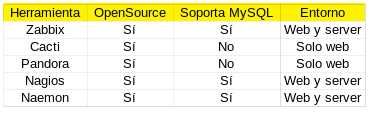
\includegraphics[scale=0.4]{imagenes/comparativanaemon.png}
	\caption{Comparativa a nivel de sistema } \label{comparativa1}
\end{figure}
Como se puede observar, Nagios y Naemon cuentan con mejores características a nivel sistema operativo, ya que se pueden configurar los entornos y los protocolos, que a diferencia de otras aplicaciones no disponen, por lo que se hace más manejable y útil la utilización de Nagios y Naemon.

\subsection{A nivel aplicación} 

\begin{figure}[H]
	\centering
	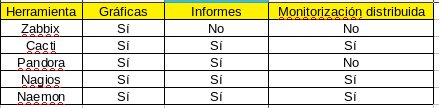
\includegraphics[scale=0.4]{imagenes/comparativanaemon2.png}
	\caption{Comparativa a nivel de aplicación } \label{comparativa2}
	
\end{figure}
\newpage
La visualización mediante gráficas, permite el poder visualizar en tiempo real todas las alertas que van apareciendo, exposición de la información de los chequeos mediante gráficas, para poder visualizar en tiempo real las alertas que van a apareciendo en el sistema. 
\subsection{A nivel extensiones} 
\begin{figure}[H]
	\centering
	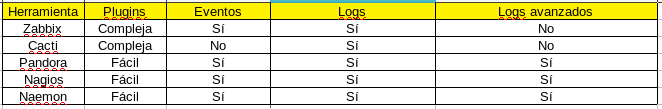
\includegraphics[scale=0.4]{imagenes/comparativanaemon3.png}
	\caption{Comparativa a nivel de extensiones } \label{comparativa3}
	
\end{figure}
Como conclusión de las posibles herramientas que dan solución a algunos de
los problemas que se están valorando, hay que destacar que existen varias que
dan solución a algunos de los problemas, pero no al mismo nivel al que se
pretende llegar, que con Nagios o Naemon se puede fácilmente. 

A la hora de realizar la selección de la herramienta entre las que hemos comentado anteriormente, cabe destacar que todas cumplen con las necesidades que pueda surgir en cualquier red a monitorizar. Por lo que para seleccionar una, se ha decidido tomar como referencia que \textbf{Naemon} se trata de un fork de Nagios, por lo que contará con todas las funcionalidades de éste, además  de contar con  un mejor rendimiento, un funcionamiento más estable y, sobre todo, una nueva interfaz gráfica mucho más ligera, moderna y rápida.  Esta nueva interfaz de Naemon, llamada, \textbf{Thruk Monitoring Webinterface}, es mucho más rápida, moderna y práctica respecto a la que aporta la suite Nagios.

\section{Introducción de Naemon}
\subsection{Funcionamiento Naemon} 
Como se ha mencionado anteriormente Naemon está basado en Nagios exactamente en la \textbf{versión 4.0.2}, el cual cumple su misma función el poder representar la monitorización del sistema, a través de los host y servicios que queramos especificar, teniendo información sobre los cambios mediante las alertas que ofrece este sistema, además de informar cuando la situación empeora o mejora.\cite{naemon}

\textbf{Naemon} se compone de dos partes, \textbf{Naemon Core y la interfaz de monitorización de Thruk}, hablaremos de ella más adelante en este capítulo, aunque es posible aplicar otra interfaz de monitorización, en todo el despliegue del proyecto se aplicará el uso de esta interfaz.

Entre las características que incluye Naemon podemos encontrar:
\begin{itemize}
	\item Monitorización de servicios de red como SMTP, POP3, HTTP, NNTP, PING, entre otros.
	\item Monitorización de los recursos del host como puede ser la carga del procesador, el uso del disco, etc.
	\item Diseño de archivos plugins que permiten a los usuarios desarrollar fácilmente sus propios controles de servicio.
	\item Controles de servicios paralelos.
	\item Thruk Monitoring Webinterface para editar la configuración y ver el estado actual de la red, el historial de problemas, los archivos de registro, los informes de sla, los paneles de control, los procesos empresariales, etc.
	\item Capacidad para definir la jerarquía de hosts de la red mediante hosts "principales", lo que permite la detección y distinción entre los hosts que están inactivos y los que no están disponibles.
	\item Avisos de contacto cuando se producen problemas con el servicio o el host y se resuelven.
	\item Capacidad para definir controladores de eventos que se ejecutarán durante el servicio o eventos de host para la resolución proactiva de problemas.
	\item Rotación automática de archivos de registro.
	\item Soporte para implementar hosts de monitoreo redundantes.
\end{itemize}

Para la monitorización de hosts y servicios, Naemon al igual que Nagios utiliza \textbf{plugins}. Se tratan de componentes externos a los que Naemon les pasa información sobre el cometido que debe realizar, es decir, lo que debe comprobarse y los límites críticos y de advertencia. Una vez sea transmitida dicha información, los plugins harán las respectivas comprobaciones y analizarán los resultados.
\newpage
Dicho resultado del chequeo podrá tener cuatro resultados: \textbf{OK, WARNING, CRITICAL y UNKNOWN}, además de información detallada de los mismos. Así de esta manera Naemon además de encontrar o notificar problemas, previene a cualquier organización que lo implemente, para no tenerlos en un futuro.

Toda esta información se recoge en un único servidor Naemon y así se puede acceder a toda la información de la infraestructura desde una única máquina.
\subsubsection{Archivo de configuración principal}
El archivo de configuración principal contiene una serie de directivas que afectan el funcionamiento del daemon de \textbf{Naemon-core}. Este archivo de configuración es leído tanto por el demonio \textbf{Naemon} como por \textbf{Thruk}, anteriormente conocido como \textbf{$"CGIs"$}. Thruk proporciona una forma sencilla de editar la configuración de Naemon en la interfaz web sin tener que usar el terminal.

El \textbf{archivo de configuración principal} es normalmente llamado \textbf{naemon.cfg} y se encuentra en la carpeta \textbf{/etc/naemon/} \cite{naemoncfg}.

\begin{figure}[H]
	\centering
	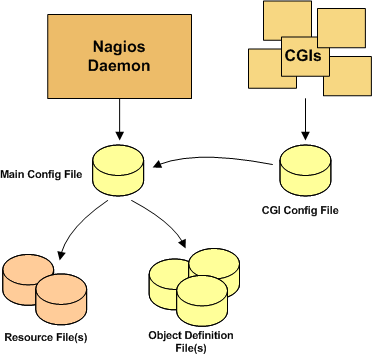
\includegraphics[width=0.7\textwidth]{imagenes/main_configuring/main_configuring.png}
	\caption{Configuración de Naemon\cite{config}}\label{configuration}
\end{figure}

La forma en la que se encuentran los \textbf{archivos de configuración de Naemon} es similar a como se encuentran en \textbf{Nagios}, al ser este un fork de él. Todo esto viene representado en la \textbf{figura \ref{configuration}.}

\subsubsection{Objetos}
La configuración de los distintos equipos y servicios a monitorizar se puede realizar a través de la carpeta \textbf{/etc/naemon/conf.d}, aquí podremos añadir equipos o hosts a la red, además podemos realizar una mejor gestión de la red.

Una de las características del formato de configuración de objetos de Naemon es que puede crear definiciones de objetos que heredan de otros.

A continuación, se explican los distintos objetos más interesantes que podemos añadir en esta \textbf{carpeta}:

\paragraph{Hosts}

Desde la carpeta \textbf{/etc/naemon/conf.d} se pueden añadir equipos a la configuración. Para ello, solo hay que crear una fichero \textbf{hosts.cfg} y además se debe conocer la dirección IP del dispositivo, el tipo de dispositivo (equipo Linux, Windows server, impresora, router o switch), sus ajustes preestablecidos, establecer los periodos de chequeo y de notificación.

A parte de esto se pueden definir relaciones entre hosts mediante el objeto \textit{\textbf{parent hosts}} que permite definir la topología de la infraestructura. Los equipos padres suelen ser routers, switches, firewalls, etc. que se encuentran entre el equipo de monitorización y
un host remoto y que se encargan de transmitir tráfico de paquetes entre ambos. Si el estado de una máquina es inaccesible puede deberse a que su \textbf{parent host},es decir, su padre original, se haya caído. \cite{naemoncfg}

Además, se pueden crear grupos que engloben a varios dispositivos que por ejemplo vayan a utilizar los mismos servicios o tengan características similares para facilitar así su monitorización y organización. El host se guardará en una base de datos.
\newpage
Uno de los principales beneficios es que esta carpeta permite a los usuarios definir plantillas y ajustes preestablecidos que pueden aplicarse al agregar hosts. Un host preestablecido contiene todos los servicios que se deben agregar a un host con todos los comandos vinculados y todos los valores predeterminados establecidos. También contiene el comando \textit{\textbf{check-host-alive}} que se aplicará al nuevo host. Al añadir un host, el usuario debe ajustar algunos parámetros para adecuar la monitorización del host a su caso específico.

Naemon viene por defecto con unas plantillas predefinidas que hacen referencia a varios posibles tipos de máquinas. En cualquier caso, y como bien se ha dicho antes, el usuario puede añadir más sistemas desde \textbf{/etc/naemon/conf.d} en la parte de additional items y advanced
items. Su formato de definición es el correspondiente a la \textbf{figura \ref{define-hosts}.}
\begin{figure}[H]
	\centering
	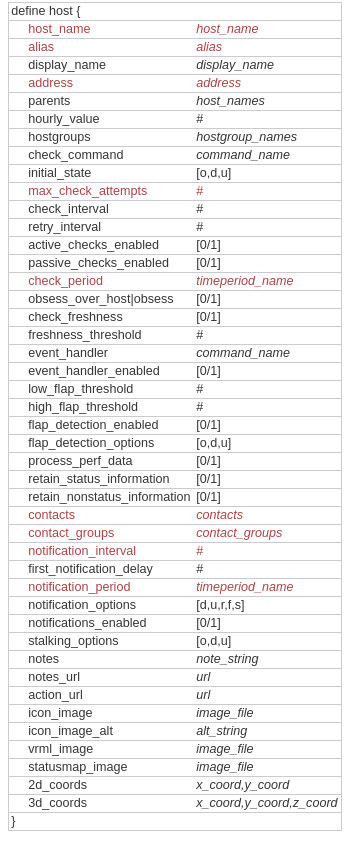
\includegraphics[scale=0.4]{imagenes/definicion_objetos/hosts.png}
	\caption{Formato de definición de un objeto de tipo Host} \label{define-hosts}	
\end{figure}
A continuación se va explicar las distintas directivas que se pueden encontrar a la hora de definir un host:
\begin{itemize}
	\item \textbf{host\_name}: se usa para definir el identificador del host con un nombre corto.
	\item \textbf{alias}: se usa para definir un nombre o una descripción para identificar el host.	
	\item \textbf{display\_name}: se utiliza para definir un nombre alternativo que debe mostrarse en la interfaz web para este host.
	\item \textbf{address}: se utiliza para definir la dirección del host. Normalmente, esta es una dirección IP, aunque realmente podría ser cualquier cosa que desee. 
	\item \textbf{parents}: se utiliza para definir una lista delimitada por comas de nombres cortos de los \textbf{hosts principales} para este host en particular.
	\item \textbf{hostgroups}: se utiliza para identificar los nombres cortos de los grupos de hosts a los que pertenece el host.
	\item \textbf{check\_command}: se usa para especificar el nombre corto del comando que se debe usar para verificar si el host está activo o inactivo.
	\item \textbf{initial\_state	[o,d,u]}: por defecto, Naemon asumirá que todos los hosts están en estado UP cuando se inicia. Puede anular el estado inicial de un host utilizando esta directiva. \textit{Las opciones válidas son: o = ARRIBA, d = ABAJO, y u = INACTIVO.}
	\item \textbf{max\_check\_attempts}: se utiliza para definir la cantidad de veces que Naemon volverá a intentar el comando de verificación de host si devuelve cualquier estado que no sea OK. Establecer este valor en 1 hará que Naemon genere una alerta sin volver a intentar la verificación del host.	
	\item \textbf{check\_interval}: se utiliza para definir el número de `unidades de tiempo'  entre las comprobaciones programadas regularmente del host.	
	\item \textbf{retry\_interval}: se utiliza para definir el número de `unidades de tiempo' que debe esperar antes de programar una nueva verificación de los hosts. 	
	\item \textbf{active\_checks\_enabled}: se utiliza para determinar si las comprobaciones activas de este host están habilitadas. 
	\item \textbf{passive\_checks\_enabled}: se utiliza para determinar si las comprobaciones pasivas están habilitadas o no para este host. 	
	\item \textbf{check\_period}: se utiliza para especificar el nombre corto del período de tiempo durante el cual se pueden realizar verificaciones activas de este host.	
	\item \textbf{process\_perf\_data}: se utiliza para determinar si el procesamiento de datos de rendimiento está habilitado o no para este host.	
	\item \textbf{event\_handler\_enabled}:	se utiliza para determinar si el controlador de eventos para este host está habilitado o no. 
	\item \textbf{retain\_status\_information}: se utiliza para determinar si la información relacionada con el estado del host se retiene o no en los reinicios del programa.	
	\item \textbf{retain\_nonstatus\_information}: se utiliza para determinar si la información que no es de estado sobre el host se retiene en los reinicios del programa. Esto solo es útil si ha habilitado la retención de estado utilizando la direc	
	\item \textbf{contacts}: Esta es una lista de los nombres cortos de los contactos que se deben notificar siempre que haya problemas con este host.	
	\item \textbf{contact\_groups}: Esta es una lista de los nombres cortos de los grupos de contacto que se deben notificar siempre que haya problemas con este host.	
	\item \textbf{notification\_interval}: se utiliza para definir el número de "unidades de tiempo" que esperar antes de volver a notificar a un contacto que este servicio aún está inactivo o inaccesible.	
	\item \textbf{notification\_period}: se utiliza para especificar el nombre corto del período de tiempo durante el cual se pueden enviar notificaciones de eventos para este host a los contactos.	
	\item \textbf{notification\_options	[d,u,r,f,s]}: se utiliza para determinar cuándo se deben enviar notificaciones para el host. Las opciones válidas son una combinación de uno o más de los siguientes: d = enviar notificaciones en estado ABAJO, u = enviar notificaciones en estado NO ALCANZABLE, r = enviar notificaciones en recuperaciones (estado correcto), f = enviar notificaciones cuando se inicia el host y deja de aletear, y s = envía notificaciones cuando comienza y termina el tiempo de inactividad programado. 
	\item \textbf{notifications\_enabled}: se utiliza para determinar si las notificaciones para este host están habilitadas o no.	
\end{itemize}

\paragraph{Servicios}

El poder de esta herramienta de monitorización reside en los servicios que se pueden monitorizar. Estos pueden ser tanto servicios públicos como privados.  \cite{naemoncfg}

Un \textbf{servicio} es “\textit{público}” cuando es accesible a través de la red, ya sea en la red local o por Internet como \textbf{HTTP, POP3, IMAP, FTP y SSH}. Estos servicios y aplicaciones, así como sus protocolos, pueden ser monitorizados por Naemon sin necesidad de requerimientos de acceso especiales.

En cambio, los servicios “\textit{privados}” no pueden ser monitorizados con Naemon sin la intervención de algún agente. Ejemplos de servicios privados asociados con los equipos son la carga de CPU, uso de memoria, uso en disco, cuentas de usuarios activos, información de procesos, etc. Estos servicios privados o atributos de los equipos usualmente no son expuestos a clientes externos. Esta situación requiere que un agente intermediario sea instalado en el equipo que se desea monitorizar esa información.

Sobre los dispositivos que hemos configurado anteriormente podemos añadir diferentes servicios de monitorización. Para ver la disponibilidad de dichas máquinas es conveniente añadir a todos ellos el servicio \textbf{PING} \cite{monitoring} que \textit{nos hará saber si ese ordenador está configurado en la red y nos notificará si alguno de ellos cae en un momento dado}, es decir, \textit{permite hacer una verificación del estado de una determinada conexión o host local}. \textbf{PING} se encuentra en la mayoría de sistemas operativos incluyendo Unix y Windows. Cabe mencionar que este servicio se encuentra desactivado en Windows por defecto.

A la hora de definir servicios es obligatorio fijar unos intervalos de chequeo del servicio y de notificación de los mismos por si alguno de ellos da algún problema a la hora de ser monitorizado. Los parámetros que definen estos periodos son los mismos que en los hosts.

En los servicios también se pueden definir plantillas con una serie de servicios a monitorizar definidos para una mayor facilidad, por ejemplo, si se quieren definir dichos servicios en múltiples equipos (en vez de tener que añadir cada servicio uno a uno, se añadirían todos los servicios de una vez).

Como en el caso de las máquinas, los servicios también se pueden agrupar. Estas agrupaciones sirven para manejar de una manera más efectiva los servicios, que sea más organizado a la hora de ver la información de los mismo en las interfaces web y para configurar dependencias entre equipos.
Su formato de definición es el de la figura \ref{define-services}.
\begin{figure}[H]
	\centering
	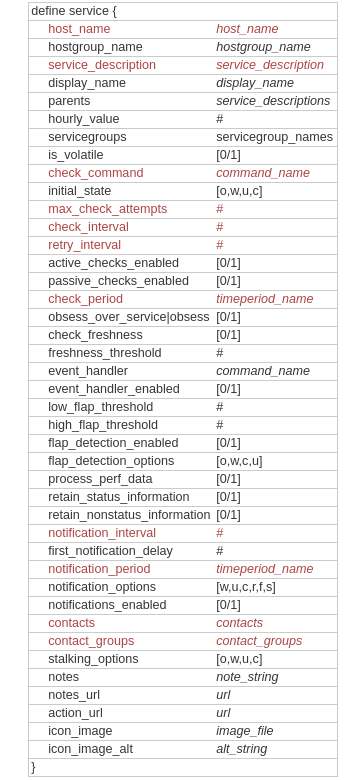
\includegraphics[scale=0.4]{imagenes/definicion_objetos/services.png}
	\caption{Formato de definición de un objeto de tipo Servicios} \label{define-services}
\end{figure}

A continuación se va explicar las distintas \textbf{directivas} que se pueden encontrar a la hora de definir un servicio, algunas son parecidas en cuanto a la funcionalidad como las usadas para definir un host:
\begin{itemize}
	\item 	\textbf{host\_name}: se utiliza para especificar los nombres abreviados de los hosts en los que el servicio se ejecuta o está asociado.	
	\item \textbf{hostgroup\_name}:	se utiliza para especificar los nombres abreviados de los grupos de hosts en los que el servicio se ejecuta" o con los que está asociado. 
	\item \textbf{service\_description}: se utiliza para definir la descripción del servicio, que puede contener espacios, guiones y dos puntos.
	\item \textbf{hourly\_value}:se utiliza para representar el valor del servicio.	
	\item \textbf{servicegroups}: se usa para identificar los nombres abreviados de los grupos de servicios a los que pertenece el servicio. Varios grupos de servicio deben estar separados por comas. 	
	\item \textbf{is\_volatile}: se utiliza para denotar si el servicio es volátil. Los servicios normalmente no son volátiles. 
	\item \textbf{check\_command}: se utiliza para especificar el nombre corto del comando que ejecutará Naemon para verificar el estado del servicio. 	
	\item \textbf{initial\_state [o,w,u,c]}: por defecto, Naemon asumirá que todos los servicios están en estado OK cuando se inicia. Puede anular el estado inicial de un servicio utilizando esta directiva. Las opciones válidas son: o = OK, w = ADVERTENCIA, u = DESCONOCIDO, y c = CRÍTICO.
	\item \textbf{max\_check\_attempts}:se utiliza para definir la cantidad de veces que Naemon volverá a intentar el comando de verificación de servicio si devuelve cualquier estado que no sea OK. 	
	\item \textbf{check\_interval}: se utiliza para definir el número de \textit{unidades de tiempo} a esperar antes de programar la próxima verificación \textit{regular} del servicio	
	\item \textbf{retry\_interval}:se utiliza para definir el número de \textit{unidades de tiempo} a esperar antes de programar una nueva verificación del servicio.	
	\item \textbf{active\_checks\_enabled}: se utiliza para determinar si las comprobaciones activas de este servicio están habilitadas o no. 	
	\item \textbf{passive\_checks\_enabled}: se usa para determinar si las comprobaciones pasivas de este servicio están habilitadas o no	
	\item \textbf{check\_period}: se utiliza para especificar el nombre corto del período de tiempo durante el cual se pueden realizar verificaciones activas de este servicio.	
	\item \textbf{obsess\_over\_service$|$obsess}: determina si las comprobaciones para el servicio estarán \textit{sobrecargadas} con el uso del comando \textit{ocsp\_command}.
	\item \textbf{check\_freshness}: se utiliza para determinar si las comprobaciones de actualización están habilitadas o no para este servicio. 	
	\item \textbf{freshness\_threshold}: se utiliza para especificar el umbral de actualización (en segundos) para este servicio. 	
	\item \textbf{event\_handler}: se utiliza para especificar el nombre corto del comando que debe ejecutarse cada vez que se detecta un cambio en el estado del servicio. 	
	\item \textbf{event\_handler\_enabled}: se utiliza para determinar si el controlador de eventos para este servicio está habilitado o no.
	\item \textbf{low\_flap\_threshold}: se utiliza para especificar el umbral de cambio de estado bajo utilizado en la detección de aletas para este servicio.  	
	\item \textbf{high\_flap\_threshold}: se utiliza para especificar el umbral de cambio de estado alto utilizado en la detección de aletas para este servicio. 	
	\item \textbf{flap\_detection\_enabled}: se utiliza para determinar si la detección de flaps está habilitada o no para este servicio.	
	\item \textbf{flap\_detection\_options	[o,w,c,u]}: se usa para determinar qué estados de servicio utilizará la lógica de detección de aletas para este servicio. Las opciones válidas son una combinación de uno o más de los siguientes: o = estados OK, w = estados de ADVERTENCIA, c = estados CRÍTICOS, u = estados DESCONOCIDOS.
	\item \textbf{process\_perf\_data}:se utiliza para determinar si el procesamiento de datos de rendimiento está habilitado o no para este servicio. 	
	\item \textbf{retain\_status\_information}: se usa para determinar si la información relacionada con el estado del servicio se retiene o no en los reinicios del programa.
	\item \textbf{retain\_nonstatus\_information}: se usa para determinar si la información que no es de estado sobre el servicio se retiene o no en los reinicios del programa.	
	\item \textbf{notification\_interval}: se utiliza para definir el número de \textit{unidades de tiempo} que esperar antes de volver a notificar a un contacto que este servicio todavía está en un estado no correcto. 	
	\item \textbf{first\_notification\_delay}: se usa para definir el número de \textit{unidades de tiempo} que esperar antes de enviar la primera notificación de problema cuando este servicio entra en un estado no correcto. 
	\item \textbf{notification\_period}: se utiliza para especificar el nombre corto del período de tiempo durante el cual se pueden enviar notificaciones de eventos para este servicio a los contactos. 
	\item \textbf{notification\_options	[w,u,c,r,f,s]}: se utiliza para determinar cuándo se deben enviar notificaciones para el servicio. Las opciones válidas son una combinación de uno o más de los siguientes: w = enviar notificaciones en estado de ADVERTENCIA, u = enviar notificaciones en estado DESCONOCIDO, c = enviar notificaciones en estado CRÍTICO, r = enviar notificaciones en recuperaciones (estado correcto), f = envía notificaciones cuando el servicio comienza y deja de aletear, y s = envía notificaciones cuando comienza y termina el tiempo de inactividad programado. 
	\item \textbf{notifications\_enabled}: se usa para determinar si las notificaciones para este servicio están habilitadas o no.	
	\item \textbf{contacts}: es una lista de los nombres cortos de los contactos que deben notificarse siempre que haya problemas con este servicio. Los contactos múltiples deben estar separados por comas.	
	\item \textbf{contact\_groups}: es una lista de los nombres cortos de los grupos de contacto que deben notificarse siempre que haya problemas con este servicio. Múltiples grupos de contacto deben estar separados por comas. 	
\end{itemize}
\paragraph{Comandos}

Los \textbf{comandos} definen cómo se deben hacer los chequeos de hosts y servicios, y cómo deben funcionar las notificaciones. Otra de sus funciones es restablecer el sistema automáticamente si es posible. \cite{naemoncfg}

La propia imagen de Naemon incluye una serie de comandos preestablecidos basados en plugins que son los que chequean los distintos servicios (SSH, HTTP, etc.) pero también el usuario puede añadir sus propios comandos.

Las definiciones  de los comandos pueden contener macros, pero se debe asegurar de incluir solo aquellas que son "validas" para las circunstancias en que se usará el comando.

A la hora de realizar la definición de un objeto de tipo \textbf{Comando} Naemon especifica una forma concreta a la hora de establecer sus directivas concretas, dicha forma viene representada en la figura \ref{define-command} donde se puede apreciar el uso de la directiva \textbf{command\_name} que se encarga de asignar un nombre al comando y \textbf{command\_line} encargada de especificar el formato de línea del comando, es decir, cómo se verá en la \textbf{shell de Naemon}. 

\begin{figure}[H]
	\centering
	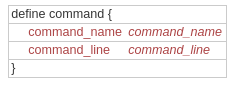
\includegraphics[scale=0.5]{imagenes/definicion_objetos/command.png}
	\caption{Formato de definición de un objeto de tipo Comandos} \label{define-command}	
\end{figure}
\newpage
\paragraph{Contactos}

Los contactos hacen referencia a diferentes personas que pueden ser los propietarios de diferentes máquinas, encargados de gestionar y solucionar problemas que pueden surgir en los dispositivos, destinatarios de notificaciones, etc.

A la hora de crear un contacto solo es obligatorio un nombre, un alias y una dirección de email. También se pueden definir los periodos de notificación de equipos y servicios y que tipo de notificaciones han de ser enviadas al contacto.

Los contactos se asignan a los usuarios que inician sesión en una de las interfaces web y todas las operaciones que se realicen a través de esa interfaz quedarán registradas como ese usuario y se permitirán dependiendo del acceso que tenga dicho usuario a determinados servicios. 

Los contactos también pueden ser agrupados en \textbf{contact groups} para dividir tareas y responsabilidades entre, por ejemplo, los empleados de una empresa. Así, por ejemplo, las notificaciones de los servicios irán destinadas a un grupo de trabajo y las de los dispositivos a otro.

Su formato de definición es el de la figura \ref{define-contact}. 
\begin{figure}[H]
	\centering
	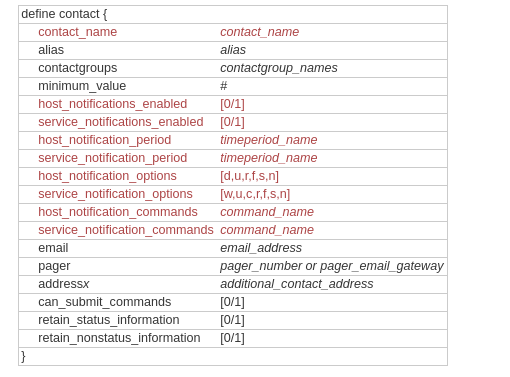
\includegraphics[scale=0.7]{imagenes/definicion_objetos/contact.png}
	\caption{Formato de definición de un objeto de tipo Contacto} \label{define-contact}
	
\end{figure}

\paragraph{Time Periods}

Los \textbf{time periods} son definiciones de periodos de tiempo en los que se pueden realizar los chequeos o se pueden enviar notificaciones de equipos y servicios. Estas definiciones se aplican a la hora de definir equipos y servicios en los parámentros check period y notification period.

Naemon trae predefinidos algún time period pero el usuario puede añadir los suyos propios. Solo hace falta un nombre único, un alias y el tiempo que se quiera definir.

Su formato de definición es el de la figura \ref{time-period}. 


\begin{figure}[H]
	\centering
	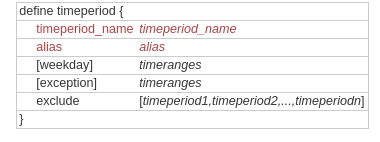
\includegraphics[scale=0.7]{imagenes/definicion_objetos/time_period.png}
	\caption{Formato de definición de un objeto de tipo Time-Period} \label{time-period}	
\end{figure}

\paragraph{Plantillas}

Como ya se ha mencionado anteriormente, Naemon permite crear \textbf{plantillas} para definir parámetros comunes que puedan ser aplicados a la hora de definir nuevos equipos y servicios.

Cuando se aplica una plantilla a un host o servicio, éste adquiere todas las propiedades definidas en la plantilla. Es posible aplicar varias plantillas a un único equipo. Si las plantillas especifican un mismo parámetro, predominará el valor del parámetro de la primera plantilla.

\subsubsection{Thruk}

\textbf{Thruk}\cite{thruk} se trata de una interfaz de monitorización \textbf{multibackend}, es decir, puede emplear una gran variedad de backends, es decir, exactamente servidores backend como es el caso de Naemon, además de herramientas como Nagios y otras muchas más, todas ellas utilizando como API la llamada \textbf{LiveStatus API} \cite{livestatus}. Está diseñado para ser un reemplazo de la herramienta y básicamente cubrir las tareas de la herramienta al completo, añadiendo grandes instalaciones y haciendo así que incrementa su usabilidad.

\textbf{Thruk} viene organizado con la siguiente estructura reflejada en la figura \ref{thruk}. Teniéndose que su autenticación HTTP viene bajo el servidor web de Apache y corriendo bajo un servidor \textbf{Fast CGI} se conecta a Naemon a través de una conexión por el puerto correspondiente a TCP/IP.

\begin{figure}[H]
	\centering
	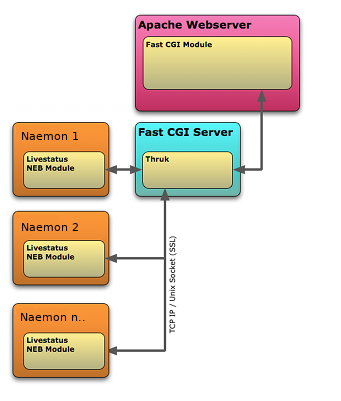
\includegraphics[scale=0.7]{imagenes/thruk/arquitectura.png}
	\caption{Estructura de conexión de Thruk} \label{thruk}
\end{figure}

A través de la página \url{https://www.thruk.org/demo.html} se puede realizar pruebas de la demo de dicha interfaz.

Entre las principales \textbf{ventajas}  de Thruk encontramos:
\begin{itemize}
	\item Múltiples backends, esto es que podemos aplicar como servidor, se pueden incluir los siguientes:\textbf{Naemon, Nagios, Icinga y Shinken}.
	Supongamos que tiene una antigua instalación de Nagios heredada aún en producción, además de un nuevo servidor Naemon o Icinga 2. Con Thruk puede configurar ambos como backends para Thruk, y le dará una vista unificada para todos los hosts y servicios configurados. Una pestaña menos en su navegador.
	\newpage
	\item Thruk tiene muchas características excelentes, pero lo primero que notas es la velocidad. Incluso una configuración con miles de hosts y decenas de miles de servicios tiene tiempos de respuesta inferiores al segundo para los listados de servicios y los resultados de búsqueda.
	\item Thruk también tiene la opción de modificar su interfaz web clásica que lo hace un poco más fácil de usar y expande la funcionalidad de monitorización e informes.
	\item Muestra en vivo la información.
	\item Fácil incorporación de plugins, tanto plugins propios de Thruk, como plugins adicionales de Naemon en este caso.	
\end{itemize}
\textbf{Thruk} viene de forma nativa con Naemon, y es una interfaz web de reemplazo completa y gratuita de código abierto para Nagios, Icinga y Shinken. Estas son herramientas flexibles para alertarnos cuando algo sale mal, y Thruk se encarga de garantizar una correcta monitorización.

Al ser una interfaz nativa de \textbf{Naemon} es preferible su utilización, puesto que su forma de integración y modificación de sus diferentes elementos será mucho menos complejo que con otras interfaces.

\subsubsection{Plugins}
A diferencia de muchas otras herramientas de monitorización, Naemon no incluye ningún mecanismo interno para verificar el estado de los hosts y servicios en su red. En su lugar, Naemon se basa en programas externos llamados \textbf{plugin} para hacer todo el trabajo.

Entonces los plugins son ejecutables o scripts (normalmente en perl, python, shell, entre otros) que se pueden ejecutar desde una línea de comandos para verificar el estado de un host o de un servicio concreto del host. Naemon usa los resultados de los plugins para determinar el estado actual de los hosts y servicios en su red. \cite{NaemonPlugins}

\textbf{Naemon} ejecutará un plugin siempre que sea necesario verificar el estado de un host o un servicio concreto del host. El plugin hace algo para realizar la comprobación y luego simplemente devuelve los resultados a Naemon. Naemon procesará los resultados que recibe del plugin y tomará las medidas necesarias.
\newpage
Los \textbf{plugins} \ref{plugin} actúan como una capa de abstracción entre la lógica de supervisión presente en el demonio de Naemon y los servicios y hosts reales que se están supervisando.

La ventaja de este tipo de arquitectura de plugins es que puede monitorear cualquier elemento.

\begin{figure}[H]
	\centering
	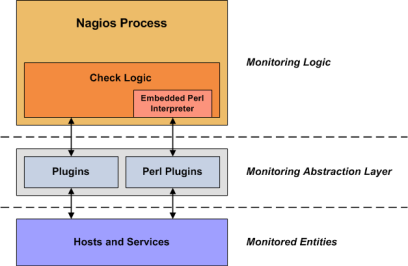
\includegraphics[scale=0.7]{imagenes/main_configuring/plugins.png}
	\caption{Funcionamiento de los plugins en Naemon} \label{plugin}	
\end{figure}

La \textbf{desventaja} de este tipo de arquitectura de plugin es el hecho de que Naemon no tiene reflejo de qué es lo que está monitorizando, simplemente rastrea los cambios en el estado de esos recursos.

Solo los plugin saben exactamente lo que están monitorizando y cómo realizar las comprobaciones reales.

Los \textbf{plugins de Naemon} no se distribuyen, pero se pueden descargar plugins de Naemon y plugins adicionales desde las siguientes \textbf{páginas}:
\begin{itemize}
	\item \textbf{Proyecto de Monitorización de Complementos: } \url{http://monitoring-plugins.org} 
	\item \textbf{Proyecto de complementos de Nagios: } \url{https://nagios-plugins.org/} 
	\item\textbf{ Nagios Exchange: } \url{http://exchange.nagios.org/}
\end{itemize}
\newpage
Hemos mencionado que Naemon se trata de un fork de Nagios, por lo que la compatibilidad y uso de sus plugins será totalmente aceptable, por lo que podemos usar cualquier plugins de la base de datos de Nagios en Naemon.